%%%%%%%%%%%%%%%%%%%%%%%%%%%%%%%%%%%%%%%%%%%%%%%%%%%%%%%%%%%%%%%%%%%%%
%%%                       ANALYSIS OVERVIEW                       %%%
%%%%%%%%%%%%%%%%%%%%%%%%%%%%%%%%%%%%%%%%%%%%%%%%%%%%%%%%%%%%%%%%%%%%%
\section{Systematic uncertainties}\label{sec:SystematicUncertainties}

We consider all the standard \gls{NOvA} systematic uncertainties grouped into four categories: neutrino flux, detector calibration, detector modelling, and neutrino interaction systematic uncertainties. Summary of the effects of both systematic and statistical uncertainties on the predicted number of \gls{SM} background events is shown in Fig.~\ref{fig:NuMMErrorBarChart}. The four categories of systematic uncertainties are assumed to be uncorrelated between each other, allowing to calculate their combined effect by adding their individual contribution in quadrature. The statistical uncertainty is calculated as $\sqrt{N_{\gls{SM}}}$ since the number of predicted events follows the Poisson distribution. The total prediction of the number of \gls{SM} background events can be expressed as
\begin{equation}
N_{\gls{SM}}=700.33 \pm 26.46\left(\textsf{stat.}\right) ^{+72.48}_{-62.99}\left(\textsf{syst.}\right).
\end{equation}

\begin{figure}[hbtp]
\centering
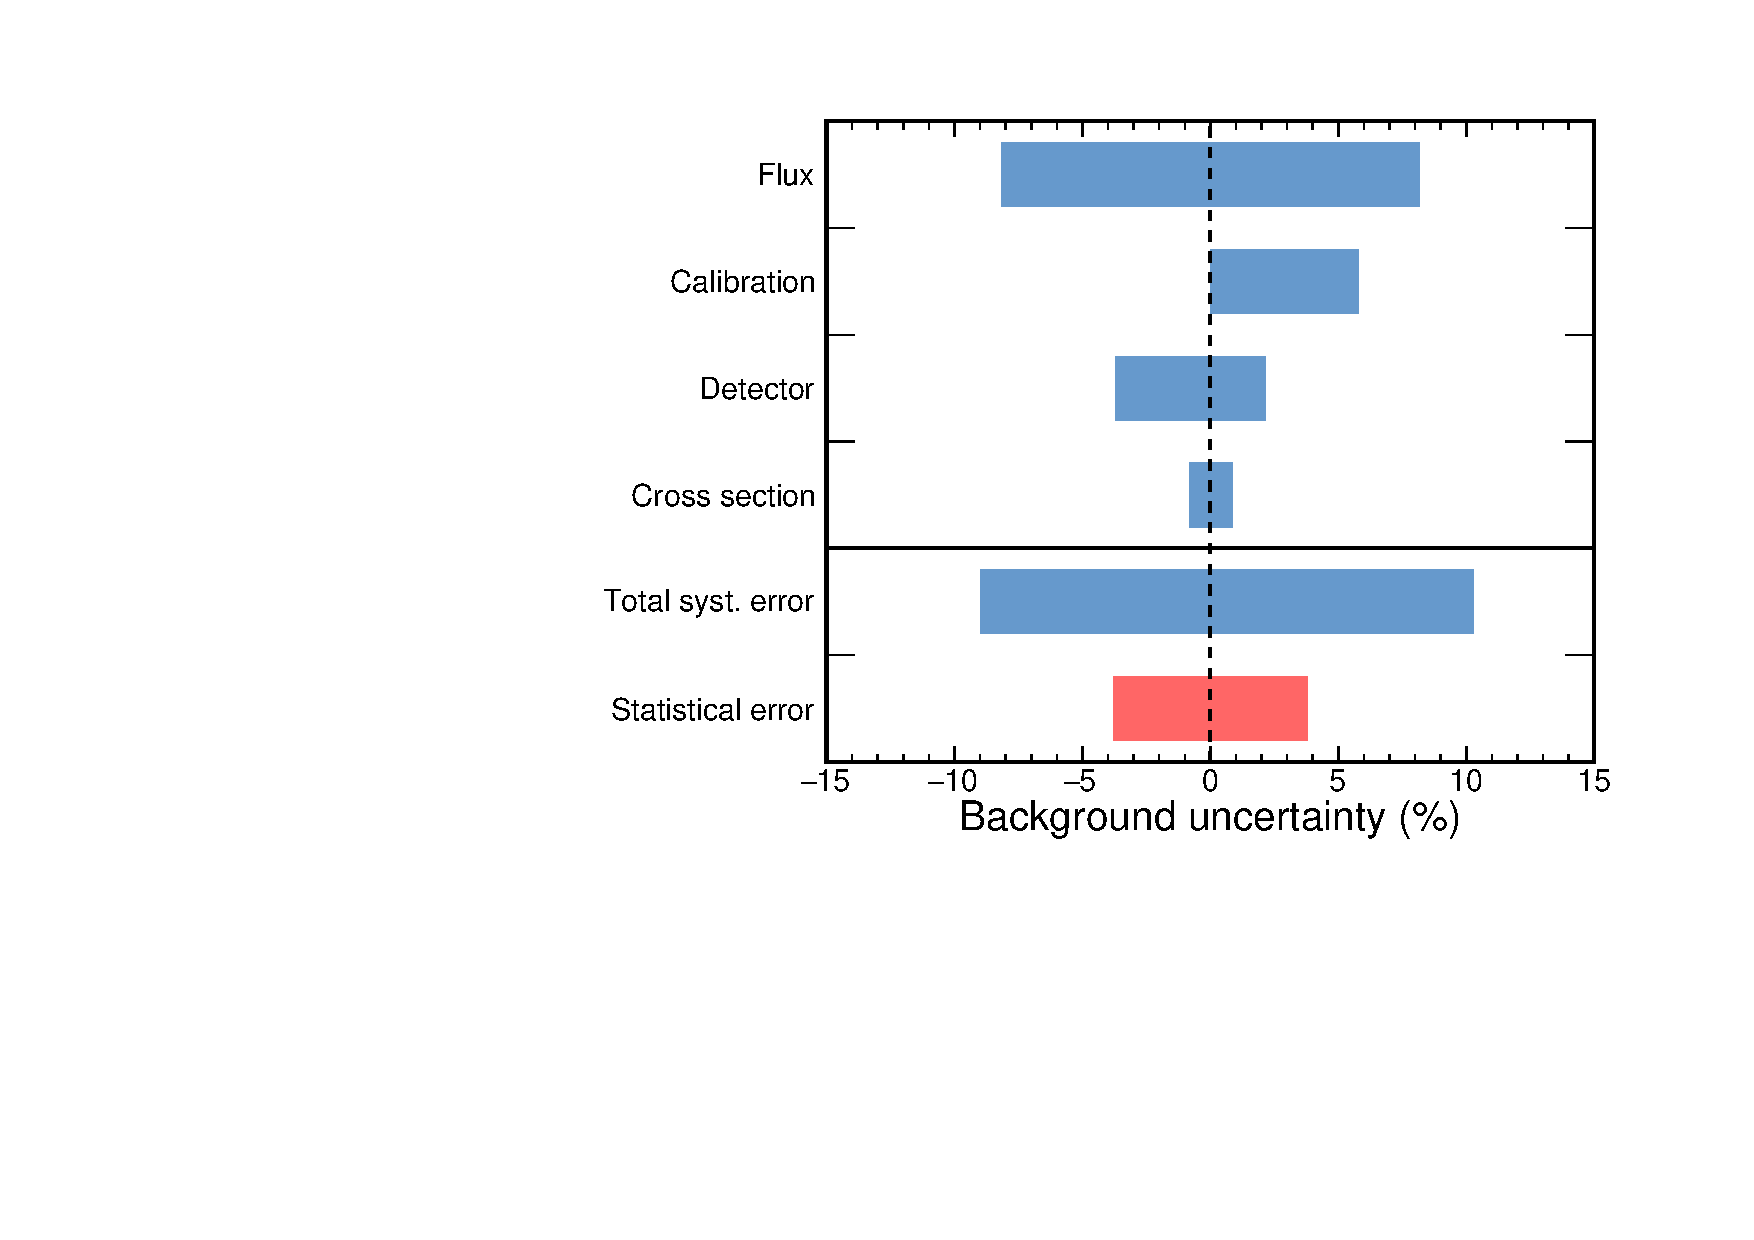
\includegraphics[width=.7\textwidth]{Plots/RelativeErrorBarChart.pdf}
\caption[Summary of systematic uncertainties]{Relative effect of systematic and statistical uncertainties on the number of \acrshort{SM} background events. The total systematic uncertainty (blue bottom bar) is calculated as a square root of the sum of squares of the four categories of systematic uncertainties, shown ordered by the size of their effect. These are the neutrino flux, detector calibration, detector modelling, and neutrino cross section systematic uncertainties.}
\label{fig:NuMMErrorBarChart}
\end{figure}

To assess the effect of the neutrino flux systematic uncertainty, we use 8 \gls{ND}-only principal components. Figure~\ref{fig:NuMMFluxSysts} shows their combined effect on the predicted \gls{SM} background as a function of the primary shower's reconstructed energy. Since the principal components are uncorrelated by construction, the total systematic uncertainty for each bin is calculated by adding the effect of all the principal components in quadrature. The effect of the neutrino flux systematic uncertainty does not depend on the primary shower's calorimetric energy and altering the neutrino flux prediction can be represented by a normalization shift. The final effect of the neutrino flux systematic uncertainty on the total number of \gls{SM} background events is $\pm\unit[8.16]{\%}$ and is symmetric around the nominal prediction.

\begin{figure}[hbtp]
\centering
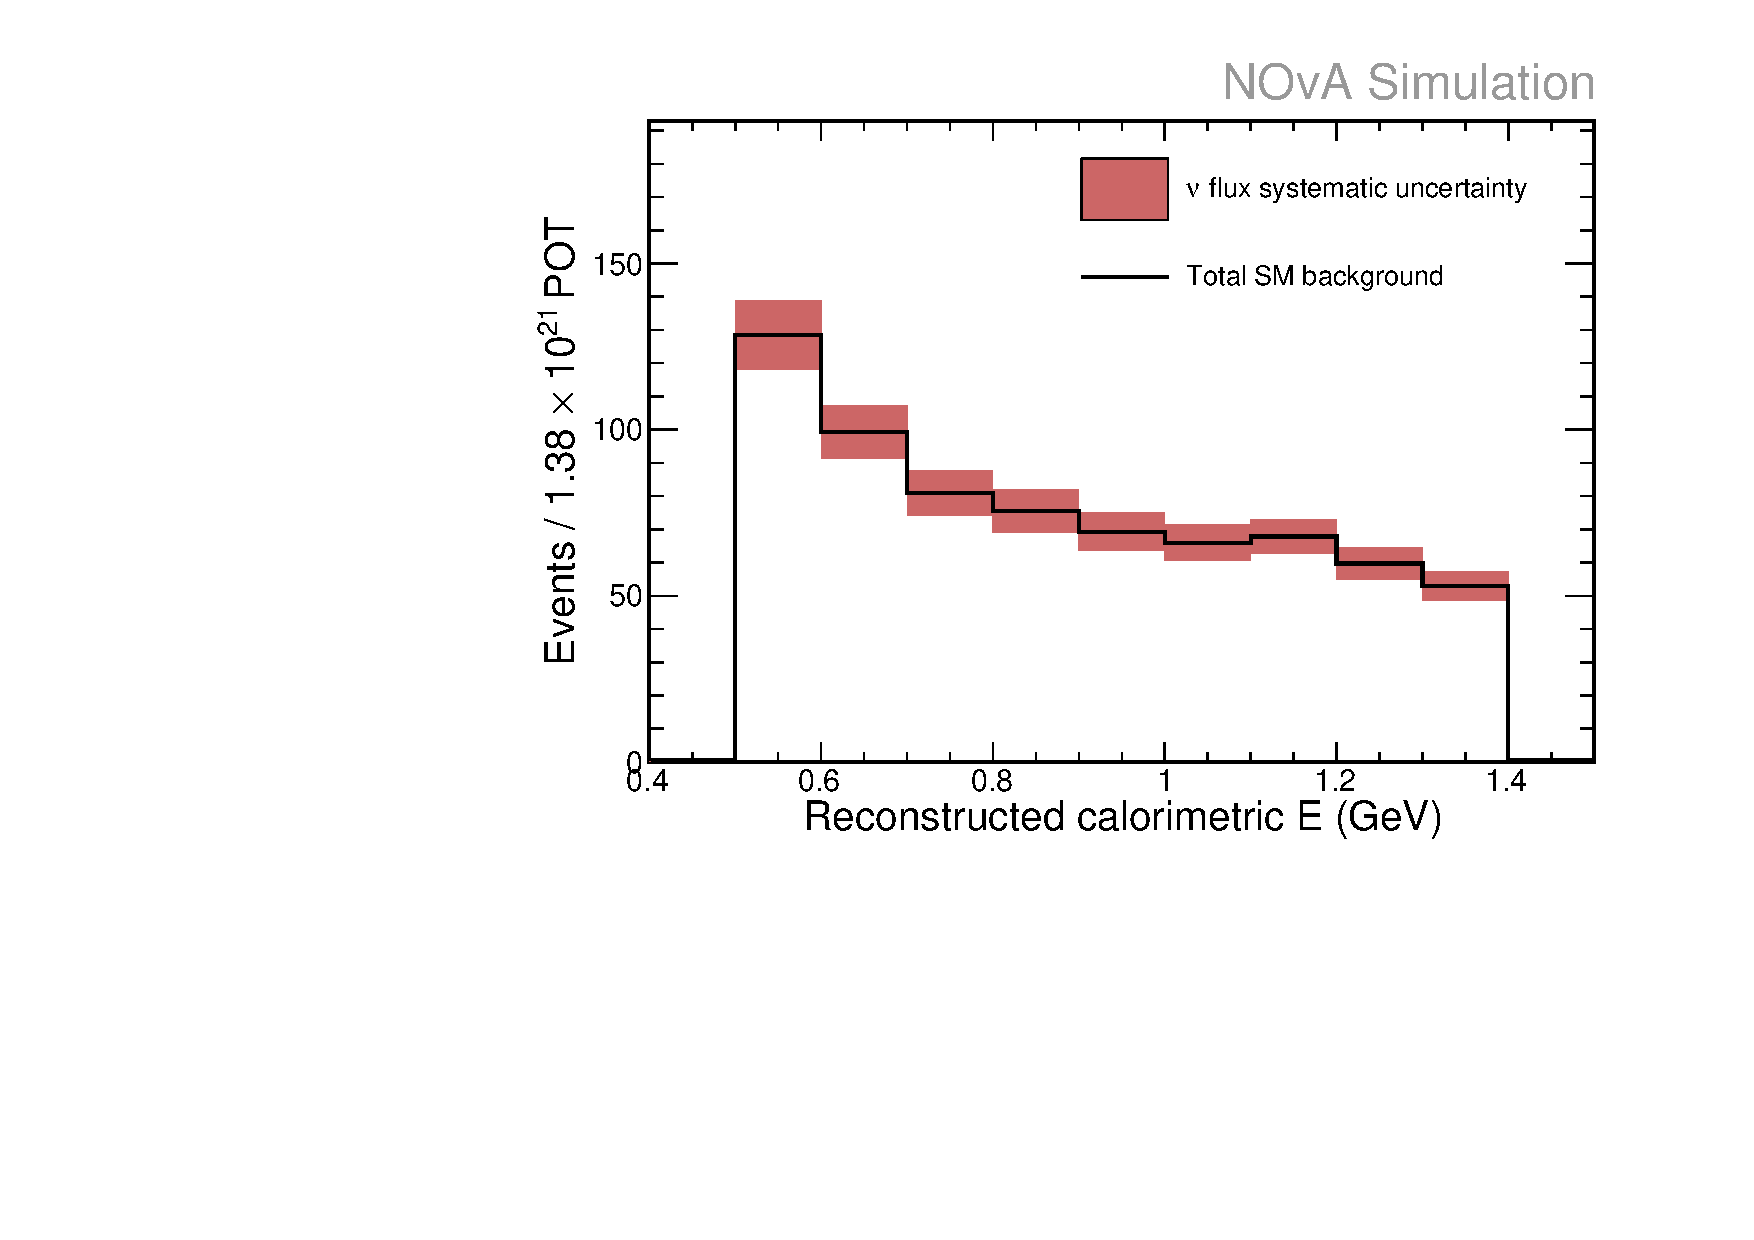
\includegraphics[width=.7\textwidth]{Plots/SystShifts_beamSysts_Full_Graph.pdf}
\caption[Neutrino flux systematic uncertainty]{Effect of the total neutrino flux systematic uncertainty on the primary shower energy distribution of the \acrshort{SM} background events.}
\label{fig:NuMMFluxSysts}
\end{figure}

The effect of the total detector modelling and calibration systematic uncertainties on the number of \gls{SM} background events is asymmetrical, increasing the number of events by $+\unit[6.17]{\%}$ and decreasing by $\unit[3.69]{\%}$. The effect of these uncertainties dependents on the energy of the primary shower (which is the recoil electron for \gls{nuone} events), as can be seen in Fig.~\ref{fig:NuMMDetSysts}. This means that the energy distribution of the \gls{SM} background events can be significantly altered due to the detector uncertainties. The largest contribution comes from the absolute energy scale uncertainty, which has a one-sided effect of $\unit[+5.72]{\%}$. This is due to both the positive and the negative shift in the absolute energy scale increasing the total number of \gls{SM} background events. The light level and  Cherenkov systematic uncertainties are asymmetrical and alter the number of \gls{SM} background events in both directions by $^{+\unit[1.13]{\%}}_{\unit[-3.39]{\%}}$ and $^{\unit[+1.82]{\%}}_{\unit[-1.46]{\%}}$ respectively. The detector ageing and calibration shape systematic uncertainties are one sided by default and increase the number of the \gls{SM} background events by $\unit[+0.55]{\%}$ and $\unit[+0.69]{\%}$ respectively.

\begin{figure}[hbtp]
\centering
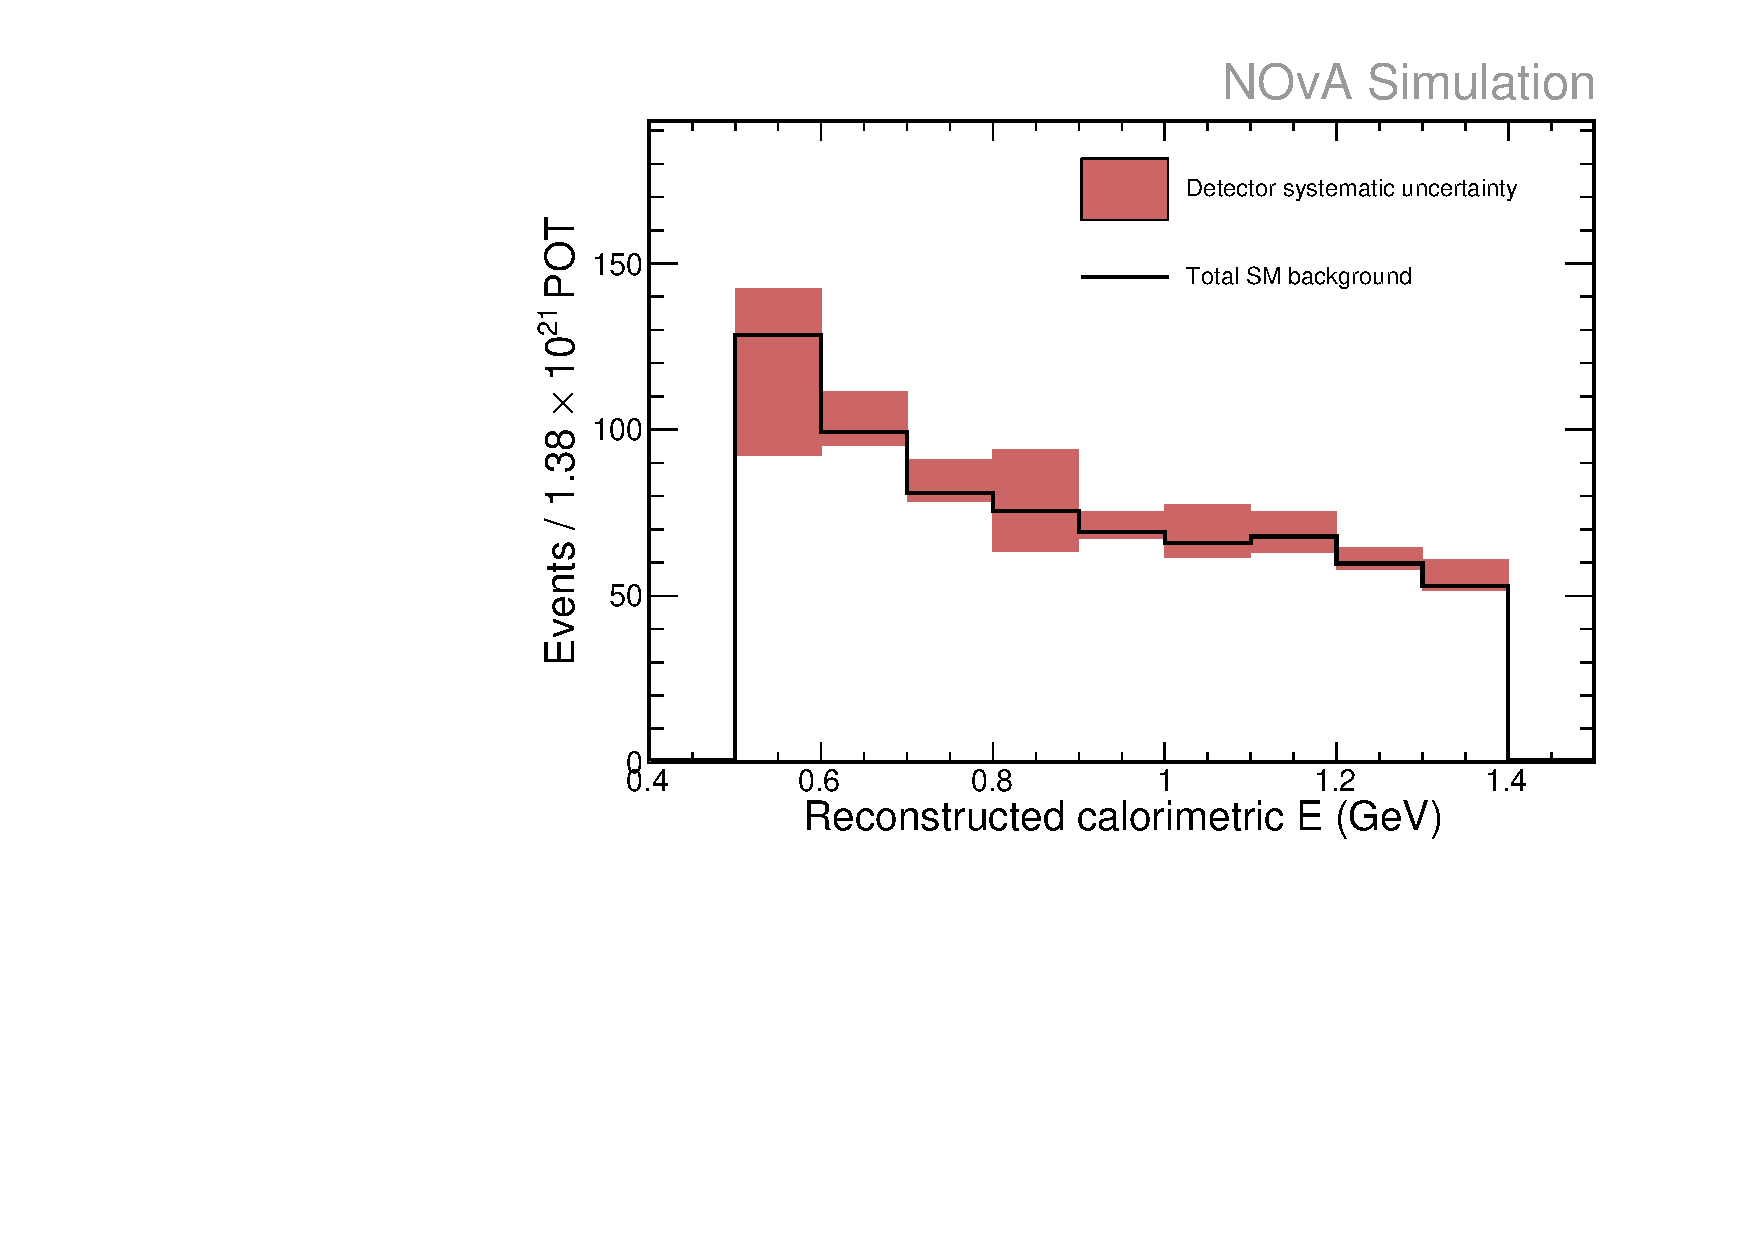
\includegraphics[width=.7\textwidth]{Plots/SystShifts_detSysts_Full_Graph.pdf}
\caption[Detector systematic uncertainties]{Effect of the total detector systematic uncertainty on the primary shower energy distribution of the \acrshort{SM} background. The detector uncertainty consists of the absolute calibration, calibration shape, detector ageing, light level, and Cherenkov systematic uncertainties.}
\label{fig:NuMMDetSysts}
\end{figure}

Since we assume that the \gls{nuone} interaction is known precisely, the dominant \gls{nuone} component of the \gls{SM} background has no systematic uncertainty from neutrino interactions. Therefore, the neutrino interaction systematic uncertainty affects only the $181$ "Other background" events, which make up $\unit[34.9]{\%}$ of the total \gls{SM} background. Consequently, the total neutrino interaction uncertainty on the \gls{SM} background is relatively small, with a combined effect on the number of \gls{SM} background events of $^{+\unit[1.54]{\%}}_{-\unit[1.49]{\%}}$.
The most dominant neutrino interaction systematic uncertainties are related to interactions with $\pi^0$ in the final state,  such as the axial mass ($^{\unit[+0.97]{\%}}_{\unit[-0.90]{\%}}$) and the vector mass ($^{\unit[+0.41]{\%}}_{\unit[-0.35]{\%}}$) of the \gls{NC}\gls{Res} interactions, the scaling of the \gls{COHpi}\gls{NC} interactions ($^{\unit[+0.85]{\%}}_{\unit[-0.85]{\%}}$), or the mean free path of pions before they undergo an interaction ($^{\unit[+0.30]{\%}}_{\unit[-0.43]{\%}}$). Other neutrino interaction systematic uncertainties have only a marginal ($<\unit[0.3]{\%}$) effect on the number of \gls{SM} background events.

%The most dominant neutrino interaction systematic uncertainties are from the axial and vector masses of the \gls{NC}\gls{Res} interaction ($^{\unit[+0.97]{\%}}_{\unit[-0.90]{\%}}$ for axial and $^{\unit[+0.41]{\%}}_{\unit[-0.35]{\%}}$ for vector mass). Also significant is the effect of the coherent \gls{NC} scaling ($^{\unit[+0.85]{\%}}_{\unit[-0.85]{\%}}$), of the \gls{QE} normalization factor ($^{\unit[+0.31]{\%}}_{\unit[-0.24]{\%}}$), or of the mean free path of pions before they undergo an interaction ($^{\unit[+0.30]{\%}}_{\unit[-0.43]{\%}}$).


%Other uncertainties have only a very small impact. The ones that have an effect of $\left(>\pm\unit[0.1]{\%}\right)$ are the suppression of long-range nuclear effect and \gls{Res} events at low energy transfers, shape of the \gls{MEC} tuning dependent on the neutrino energy, single $\pi$ \gls{NC}\gls{DIS} production, distance parton travels before hadronization, axial mass of \gls{NC} elastic and \gls{CC}\gls{Res} interactions, branching ratios of radiative and $\eta$-resonance decays, or the $\pi$ angular distribution in the $\Delta$ resonance decays.

\iffalse
The largest systematic uncertainty for neutrino interaction comes from:
MaNCRES (0.97\%, -0.90\%) axial mass for NC resonant neutrino production $\pm\unit[20]{\%}$ - from GENIE,
MvNCRES (+0.41\%, -0.35\%) vector mass for NC resonant neutrino production $\pm\unit[10]{\%}$ - from GENIE,
COHNCScale208 (+0.85\%, -0.85\%),
ZNormCCQE (+0.31\%, -0.24\%) is the Z-expansion normalization and represents a $\unit[+20]{\%}/\unit[-15]{\%}$ QE normalization factor - GENIE,
hNFSI\_MFP\_2024 (+0.30\%, -0.43\%) the mean free path (mean distance traveled by) of pions before they undergo an interaction

Other notable $\left(>\pm\unit[0.1]{\%}\right)$ contributions are from (in no particular order)
RPAShapesupp2020 (how well is the RPA understood, this one suppresses it at low $Q^2$),
LowQ2RESSupp2020 (one sided uncertainty due to an observed discrepancy at low $Q^2$ of RES events in NOvA data),
MECShape2024Nu (neutrino energy dependence of the MEC fit), DISvpNC2pi\_2020 (normalization uncertainty for transition-DIS events, starting at $\unit[50]{\%}$ at high $W\leq\unit[3]{GeV}$ to $\unit[5]{\%}$ at $\unit[5]{GeV}$ - implemented individually for different number of $\pi$ and CC and NC),
DISvnNC1pi\_2020 (same as the previous one),
DISNuHadronQ1Syst, FormZone2024 (distance that a parton travels before hadronization),
MaNCEL (axial mass of NC elastic interactions $\pm\unit[25]{\%}$ - GENIE),
MaCCRES (axial mass for CC resonant interactions $\pm\unit[20]{\%}$ - GENIE),
RDecBR1gamma (branching ratio for radiative decays by $\pm\unit[50]{\%}$ - GENIE),
RDecBR1eta (tweaks the branching ratio of single $\eta$ decay by 50\% - the decay $R\rightarrow X+\eta$ - GENIE),
Theta_Delta2Npi (distorts the $\pi$ angular distribution in the decay $\Delta\rightarrow N+\pi$)
\fi